\chapter{Research}

\label{research}

\section{Introduction}

The use of image processing and it's associated computational techniques for the analysis, enhancement, compression and reconstruction of images has been used in the medical domain since the late 1960's and early 1970's to develop an understanding of the processes and composition of the Human Body \cite{HansonHistory}. 
More recently, technological innovations in the area of determining body composition accurately have become more mature \cite{WeyersBodpod} and thus more relevant to the study of the human body as health conditions and the research of disease behaviour has been identified as being dependent on the body's internal composition \cite{SteinkampComposition}. 
Techniques that use MRI scanning or other radiation based techniques offer significant insight into the composition of the body's internal structure. 
Particular studies have utilised whole body MRI scanning to produce images that can then be used to determine composition due to it's large coverage, low impact and ability to repeatedly acquire images \cite{KullbergMRI}. 

Image processing has also been used as a means of calibrating the scanning procedure for patients who require repeated ultrasound or other similar non-intrusive scans of a particular area of the body during a course of treatment or for the diagnosis or analysis of a course of therapy or weight loss programme. 
Previous research has provided the basis for markerless recognition by using points of reference on the human body for automated feature extraction \cite{LeongMarkerless}. 
The identification of the components of the human body without markers forms the basis for our research into the identification of sites for ultrasound scanning without the use of significant cues or markers.

Range Imaging, especially HDR is a relatively new technique being used in the context of image processing. 
Range Imaging produces 2D images with depth cues and while their relative applications in Medical Imaging have been small to date their potential is evident in previous applications outside of the context of medicine with pixel values corresponding to distance from the device already being used in the calibration of patient positioning for MRI scans using range imaging sensor devices.

This research section will consider the use of Body Composition in the analysis and diagnosis of medical state and conditions that a patient may be subject to. 
It will consider the current standards for the determination and analysis of Body Composition and what the future direction of image processing for the determination of body composition is.
Markerless recognition in the context of scan registration and patient calibration will also be explored and technologies and practices identified where the standards are implemented. 
Range Imaging techniques and devices will also be introduced within the context of these previous two medical sub-domains in order to inform our research into related work and project design and implementation.

\section{Body Composition}

The composition of the human body as determined by the physical fitness of a person is the relative percentages of fat, muscle, bone and other tissues in the body. 
This ratio of muscle to fat tissue is typically responsible for the outward appearance of a person and determines their leanness with respect to their body fat percentage. 
Body mass and volume is most commonly determined using the Body Mass Index (BMI) and this measurement has been used in clinical trials for a number of years in the determination of health conditions and disease proliferation linked to a person's height and weight \cite{PrevalenceFlegal}. 
However, BMI is limited by the lack of information that can be gained from the correlation of height and weight in the determination of mass and is unable to detect excess body adiposity of people in the intermediate range of the BMI scale who may have reasonable weight to height ratios but excessive weight distribution or abdominal volume \cite{BMIAccuracy}.

\begin{figure}[t]
\label{bmi30}
	\centering
	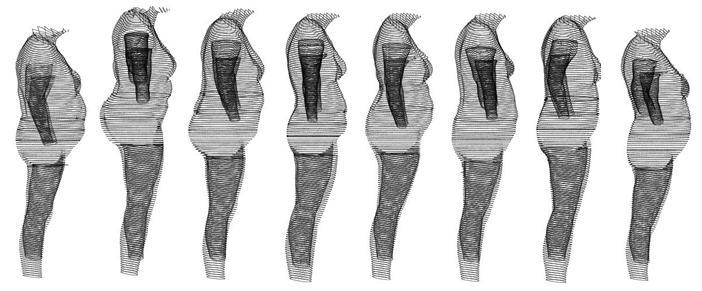
\includegraphics[scale=0.6]{images/bmi30women.jpg}
	\caption{8 Women with a BMI of 30 but with different weight distribution}
\end{figure}

A new measure of body composition is the Body Volume Index (BVI) launched in 2010 as an improved anthropometric measurement for the discovery of weight information and distribution on the human body. 
BVI is ascertained using a scanner that operates using a 3D scanner to calculate measurements and risk factors that could be associated with a person's body shape and type through the capturing of their weight, volume and body fat \cite{BVIRelease}. 
The calculation of a person's Body Volume Index in cases of obese patients was identified as being linked  to bio markers of cardiovascular disease and highlights the benefits associated with methods of acquiring 3D images of the body in the motivation of measuring patient volume for weight loss.

\section{Background Subtraction and Person Isolation}
\label{background subtraction and person isolation
In order to create a point cloud of a person, the tool kit must be able to isolate the person being scanned from the background environment. This is a well researched problem and is an issue for many applications in the computer vision field.\\
\subsection{Isolating Objects}
\label{isolating objects}


A common approach is to perform background subtraction, which identies moving objects from
the portion of a video frame that diers signicantly from a background model.

\subsection{Current Methods}

\section{Markerless Recognition}

\section{Range Imaging}

\subsection{Traditional Imaging Equipment}

\subsection{HDR Cameras}

\subsection{IR Sensors}

\subsubsection{Microsoft Kinect}

\section{Related Work}

